%! Author = antoniomasotti
%! Date = 25.11.23


\begin{frame}{Contracts}

    \begin{block}{Contracts}
        A formal agreement between parties or individual. Synonyms: pact, agreement, protocol, deal

        --- Oxford English Dictionary
    \end{block}

\end{frame}

\begin{frame}{A pact between who?}

    \only<1-2>{
    \begin{itemize}
        \item \textbf{Consumer}: the service that consumes the information (typically closer to the user)
        \item \textbf{Provider}: the service that provides the information (typically closer to the data)
    \end{itemize}
    }

    \only<2>{
    \vspace{.5cm}
    \textbf{Where do we find this architecture?}

    \begin{itemize}
        \item REST, GraphQL, gRPC, SOAP \ldots APIs
        \item Microservices communication (over TCP, HTTP, Quic, AMQP, \ldots)
        \item SOA
        \item Other kinds of distributed systems (IoT, \ldots)
        \item Client-Server
        \item Messaging systems (Kafka, RabbitMQ, SQS \ldots)
        \item Notifying systems (Webhooks, SNS, \ldots)
    \end{itemize}
    }
\end{frame}

\begin{frame}{Contract Test Role}
    \begin{center}
        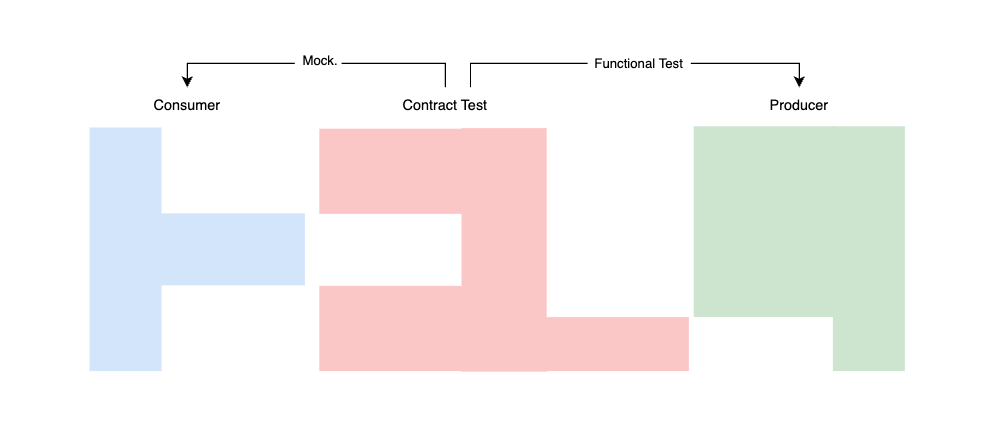
\includegraphics[scale=.3]{./assets/contract_divided}
        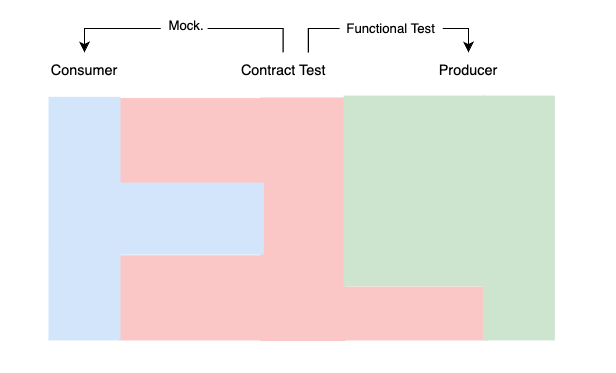
\includegraphics[scale=.3]{./assets/contract_united}
    \end{center}
\end{frame}

\begin{frame}{Who initiates the contract?}
    Both parties can initiate the contract, \textbf{but...}

    Here I will present you the \textbf{Consumer Driven Contracts} approach.
\end{frame}

\begin{frame}{Consumer Driven Contracts}
    "`\textit{A strange inversion of reasoning...}"'
    \begin{columns}
        \begin{column}{0.5\textwidth}
            \begin{itemize}
                \item Consumer Driven Contracts
                \item Pact is a contract testing tool
                \item Pact is a specification for consumer driven contracts
                \item Pact is a set of frameworks that support consumer driven contracts
            \end{itemize}
        \end{column}
        \begin{column}{0.5\textwidth}
            \begin{center}
                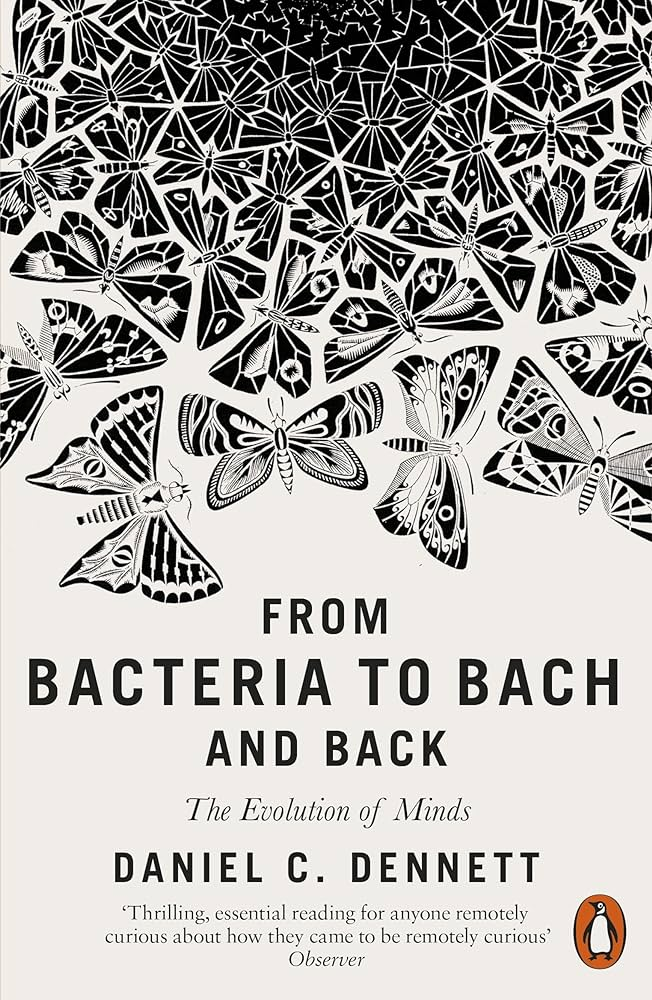
\includegraphics[width=.5\textwidth]{./assets/bacteria}
                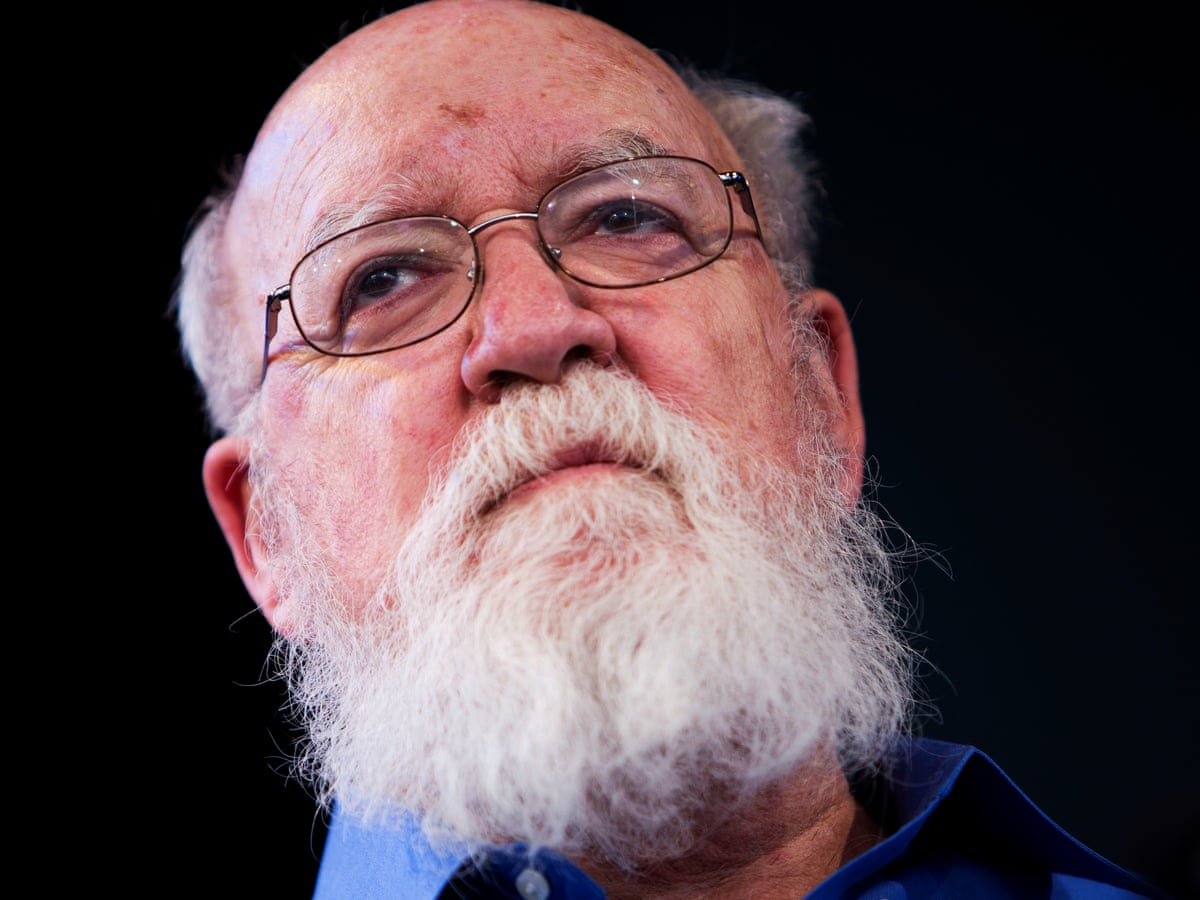
\includegraphics[width=.5\textwidth]{./assets/dennet}
            \end{center}
        \end{column}

    \end{columns}
\end{frame}


\subsection{Pact}


